\chapter{Theory}
%\label{chap:theory} this doesn't seem to work

%Theory relevant to the spectroscopy and detection of single Ba/Ba\textsuperscript{+} in SXe matrices is discussed.  Spectroscopy of Ba/Ba\textsuperscript{+} is first...

um

\section{Ba/Ba\textsuperscript{+} Spectroscopy in Vacuum}

%Some of the low-lying energy levels for Ba in vacuum are shown in Fig. \ref{fig:elevsBa}.

Transition rates for the lowest-lying energy levels in vacuum are shown in Table \ref{table:BaTransitions} for Ba and Ba\textsuperscript{+}.  um um um um um For Ba, the main transition is between the ground $6s^{2}$ $^{1}$S$_{0}$ to the excited $6s6p$ $^{1}$P$_{1}$\textsuperscript{o}, however branching ratios from the P state result in a decay to one of three metastable D states in about 1 in 330 excitations.  For Ba\textsuperscript{+}, shown in Fig. \ref{fig:elevsBaPlus}, two strong transitions exist between the ground $6s$ $^{2}$S$_{1/2}$ and the $6p$ $^{2}$P$_{1/2}$ and $6p$ $^{2}$P$_{3/2}$ excited states.  Transitions to the two metastable D states are higher than for the atom, resulting in a decay into a D state after about 4 excitations.  These D states are metastable because they are parity-forbidden to decay back to the ground state, resulting in much lower decay rates.

%These rates are shown in  along with each of the allowed transitions in Fig. \ref{fig:elevs}.

\begin{table}[!htbp]
\caption{\emph{\color{red}the 5-s one is 8 s for measurement in [11] of phys rev a 46 5 (1992), is 1/lifetime is right.}} %not sure what [Small Table], between \caption and {}, w/ no spaces, does
\label{table:BaTransitions}
\begin{tabular}{c|c|c|c}
& Transition & Rate ($s^{-1}$) & Ref. \\
\hline
Ba & $6s6p$ $^{1}$P$_{1}$\textsuperscript{o} $\rightarrow 6s^{2}$ $^{1}$S$_{0}$ & $1.19 \times 10^{8}$ & \cite{BaAllowedTransitions} \\
& $6s6p$ $^{1}$P$_{1}$\textsuperscript{o} $\rightarrow 6s5d$ $^{1}$D$_{2}$ & $2.50 \times 10^{5}$ & \cite{BaAllowedTransitions} \\
& $6s6p$ $^{1}$P$_{1}$\textsuperscript{o} $\rightarrow 6s5d$ $^{3}$D$_{2}$ & $1.1 \times 10^{5}$ & \cite{BaAllowedTransitions} \\
& $6s6p$ $^{1}$P$_{1}$\textsuperscript{o} $\rightarrow 6s5d$ $^{3}$D$_{1}$ & $3.1 \times 10^{3}$ & \cite{BaAllowedTransitions} \\
& $6s5d$ $^{1}$D$_{2} \rightarrow 6s^{2}$ $^{1}$S$_{0}$ & $5$ & \emph{\color{red}[?]} \\
& $6s5d$ $^{3}$D$_{2} \rightarrow 6s^{2}$ $^{1}$S$_{0}$ & $1.4 \time 10^{-2}$ & \emph{\color{red}[?]} \\
& $6s5d$ $^{3}$D$_{1} \rightarrow 6s^{2}$ $^{1}$S$_{0}$ & $1.7 \time 10^{-2}$ & \emph{\color{red}[?]} \\
\hline
Ba\textsuperscript{+} & $6p$ $^{2}P_{3/2}$\textsuperscript{o} $\rightarrow 6s $ $^{2}S_{1/2}$ & $1.11 \times 10^{8}$ & \cite{BaAllowedTransitions} \\
& $6p$ $^{2}P_{1/2}$\textsuperscript{o} $\rightarrow 6s$ $^{2}S_{1/2}$ & $9.53 \times 10^{7}$ & \cite{BaAllowedTransitions} \\
& $6p$ $^{2}P_{3/2}$\textsuperscript{o} $\rightarrow 5d$ $^{2}D_{5/2}$ & $4.12 \times 10^{7}$ & \cite{BaAllowedTransitions} \\
& $6p$ $^{2}P_{3/2}$\textsuperscript{o} $\rightarrow 5d$ $^{2}D_{3/2}$ & $6.00 \times 10^{6}$ & \cite{BaAllowedTransitions} \\
& $6p$ $^{2}P_{1/2}$\textsuperscript{o} $\rightarrow 5d$ $^{2}D_{3/2}$ & $3.10 \times 10^{7}$ & \cite{BaAllowedTransitions} \\
& $5d$ $^{2}D_{5/2} \rightarrow 6s$ $^{2}S_{1/2}$ & $3.8 \times 10^{-2}$ & \cite{BaPlusD52} \\
& $5d$ $^{2}D_{3/2} \rightarrow 6s$ $^{2}S_{1/2}$ & $1.3 \times 10^{-2}$ & \cite{BaPlusD32} \\
\end{tabular}
\end{table}

%The lowest-lying energy levels in vacuum for Ba and Ba\textsuperscript{+} are shown in Fig. \ref{fig:elevs}.  For Ba, the main transition is between the ground $6s^{2}$ $^{1}$S$_{0}$ to the excited $6s6p$ $^{1}$P$_{1}$\textsuperscript{o} state, however branching ratios from the P state result in a decay to one of three metastable D states in about 1 in 330 excitations.  For Ba\textsuperscript{+}, two strong transitions exist between the ground $6s$ $^{2}$S$_{1/2}$ and the $6p$ $^{2}$P$_{1/2}$ and $6p$ $^{2}$P$_{3/2}$ excited states.  Transitions to the two metastable D states are higher than for the atom, resulting in a decay into a D state after about 4 excitations.  These D states are metastable because they are parity-forbidden to decay back to the ground state, resulting in much lower decay rates.  These rates are shown in Table \ref{table:BaTransitions} along with each of the allowed transitions in Fig. \ref{fig:elevs}.

\begin{figure} %[H]
	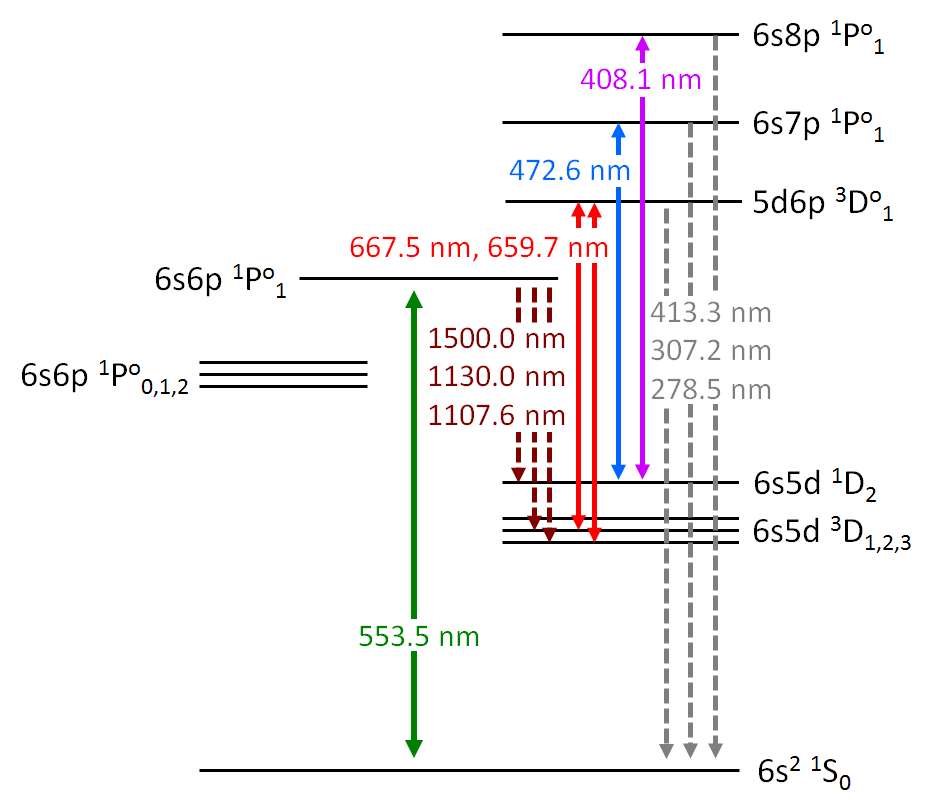
\includegraphics[width=.8\textwidth]{figures/elevs_Ba_extra.png}
	\caption{Ba energy levels in vacuum.}
    \label{fig:elevsBa}
\end{figure}

\begin{figure} %[H]
	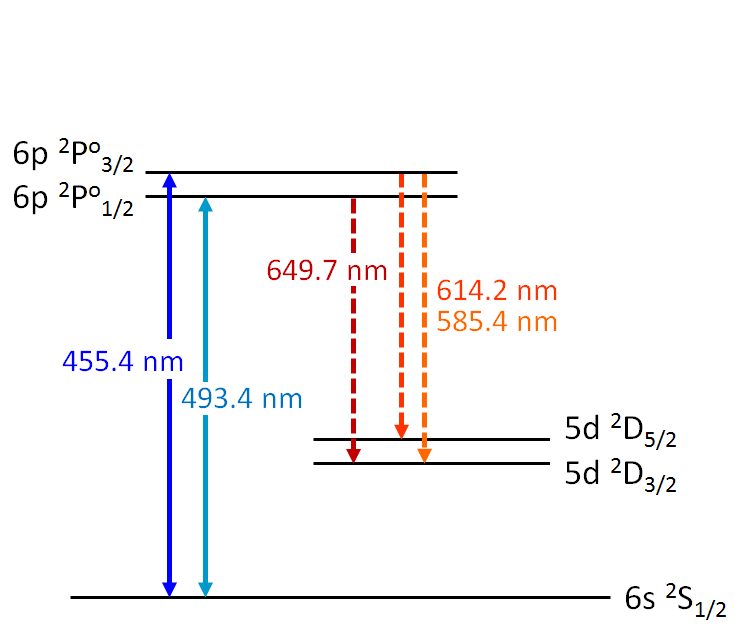
\includegraphics[width=.6\textwidth]{figures/elevs_Ba+_separate.png}
	\caption{Ba\textsuperscript{+} energy levels in vacuum.}
    \label{fig:elevsBaPlus}
\end{figure}

%\begin{figure}[H]
%	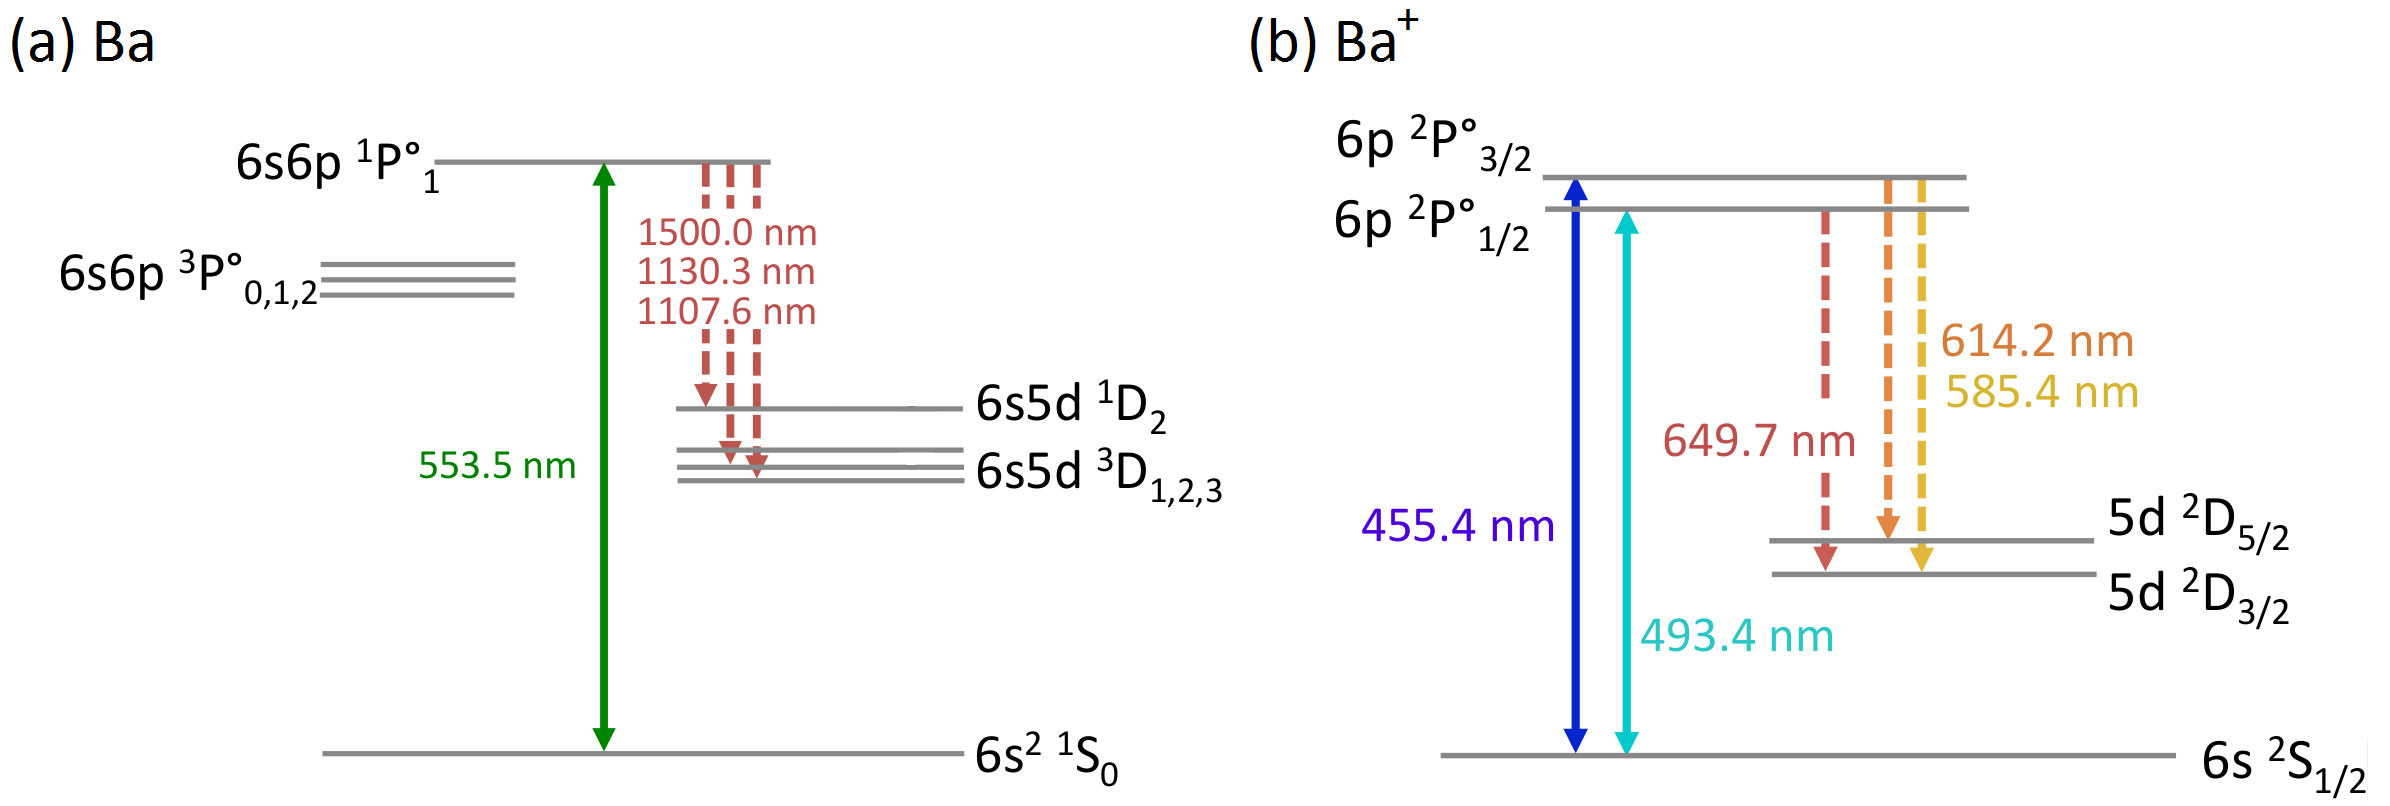
\includegraphics[width=.9\textwidth]{figures/elevs.png}
%	\caption{Energy level diagrams for (a) Ba and (b) Ba\textsuperscript{+}.}
%    \label{fig:elevs}
%\end{figure}

%These energy levels and their transition rates are well known, and are documented in the NIST Atomic Spectra Database.

Single atom/ion detection by spectroscopy generally requires, in addition to the main excitation laser, lasers to provide transitions out of the metastable D states once the atom/ion decays into one of them.  For the atom, this can be done via three additional infrared lasers for the direct transitions back to the $6s6p$ $^{1}$P$_{1}$\textsuperscript{o} state, and also via excitation to higher-level states which have paths back into the fluorescence cycle, such as $6s6p$ $^{3}$D$_{1}$\textsuperscript{o}.  Trapping/detection of Ba atoms in a magneto-optical trap (MOT) was achieved in \cite{BaMOT}.  Observation of trapped single Ba\textsuperscript{+} ions requires only two lasers if the $^{2}$P$_{1/2}$ excited state is used, e.g. \cite{singleBaPlusEXO}.

\section{Matrix Isolation Spectroscopy}

%\emph{\color{gray}May be good matrix isolation theory references in Ba Spec... yeah, 1 and 2 i think ... shon's 55, 57, 58 are probably good too and maybe overlapping}

In the matrix isolation spectroscopy technique \cite{matrixIso}, the species of interest, e.g. Ba/Ba\textsuperscript{+}, is embedded and trapped in an inert host matrix, e.g. solid Xe, ideally with a host:guest ratio of $10^{3}$ or greater for a low probability of guest-guest interaction.  The ground S state of Ba, as well as for Ba\textsuperscript{+}, is spherically symmetric, and being slightly larger in Van der Waals radius than Xe, it is likely to take the place of one or more Xe atoms in the fcc crystal (substitution), vs. existing in between Xe atoms in the crystal structure (interstitial).  However, the strength of the Ba-Xe interaction, an induced dipole-dipole Van der Waals force, is quite different when the Ba is in the non-spherically-symmetric excited P state \cite{crepin}.  This leads to significant broadening of absorption and emission for the Ba, as well as an energy shift between the two, according to the Franck Condon Principle, illustrated in Fig. \ref{fig:FranckCondon}.  In a cold matrix, the system will be in the ground lattice vibrational state ($\nu =0$) before excitation.  Electronic excitation can occur to multiple vibrational modes whose wavefunctions overlap that of the ground state, thus broadening the absorption energy.  In the excited state, rapid decay occurs to the lowest vibrational mode, and then a similar broadening in the spontaneous emission energy occurs.  A redshift in the emission is observed relative to the excitation.

% before electronic decay can occur

\begin{figure} %[H]
        \centering
                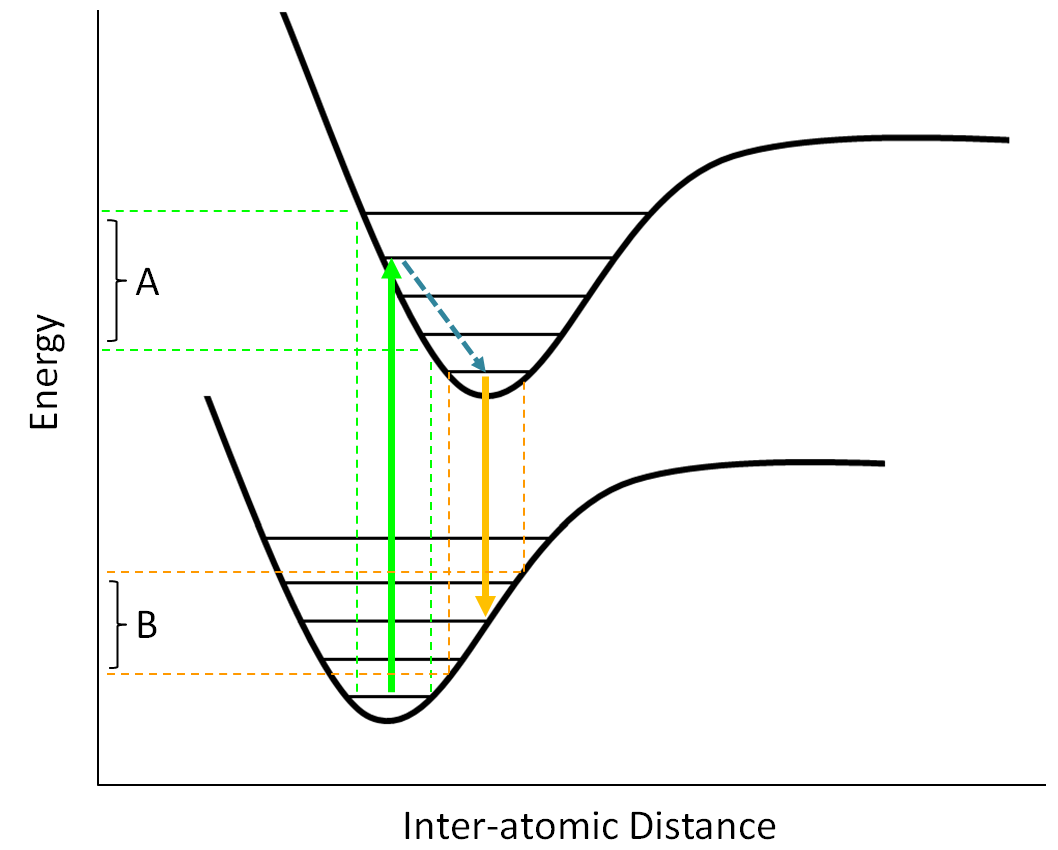
\includegraphics[width=.7\textwidth]{figures/FranckCondon.png}
                \caption{Illustration of the Franck-Condon Principle resulting in red-shifted emission as well as broadening in absorption (A) and emission (B) due to vibrational modes $\nu$ ($\nu$') in the ground (excited) state.}
\label{fig:FranckCondon}
\end{figure}

%\emph{\color{gray}Jahn-Teller?}

The spectroscopy of Ba in solid Ar (SAr) and solid Kr (SKr) matrices was studied in \cite{SAr}.  The example of Ba in SAr is shown in Fig. \ref{fig:BaSAr}.  The absorption is 10s of nm broad with a multi-peak structure, and the emission is broadened to nms and red-shifted.  These were attributed to the main $6s^{2}$ $^{1}$S$_{0} \rightarrow 6s6p$ $^{1}$P$_{1}$\textsuperscript{o} transition and its spontaneous emission.

\begin{figure} %[H]
        \centering
                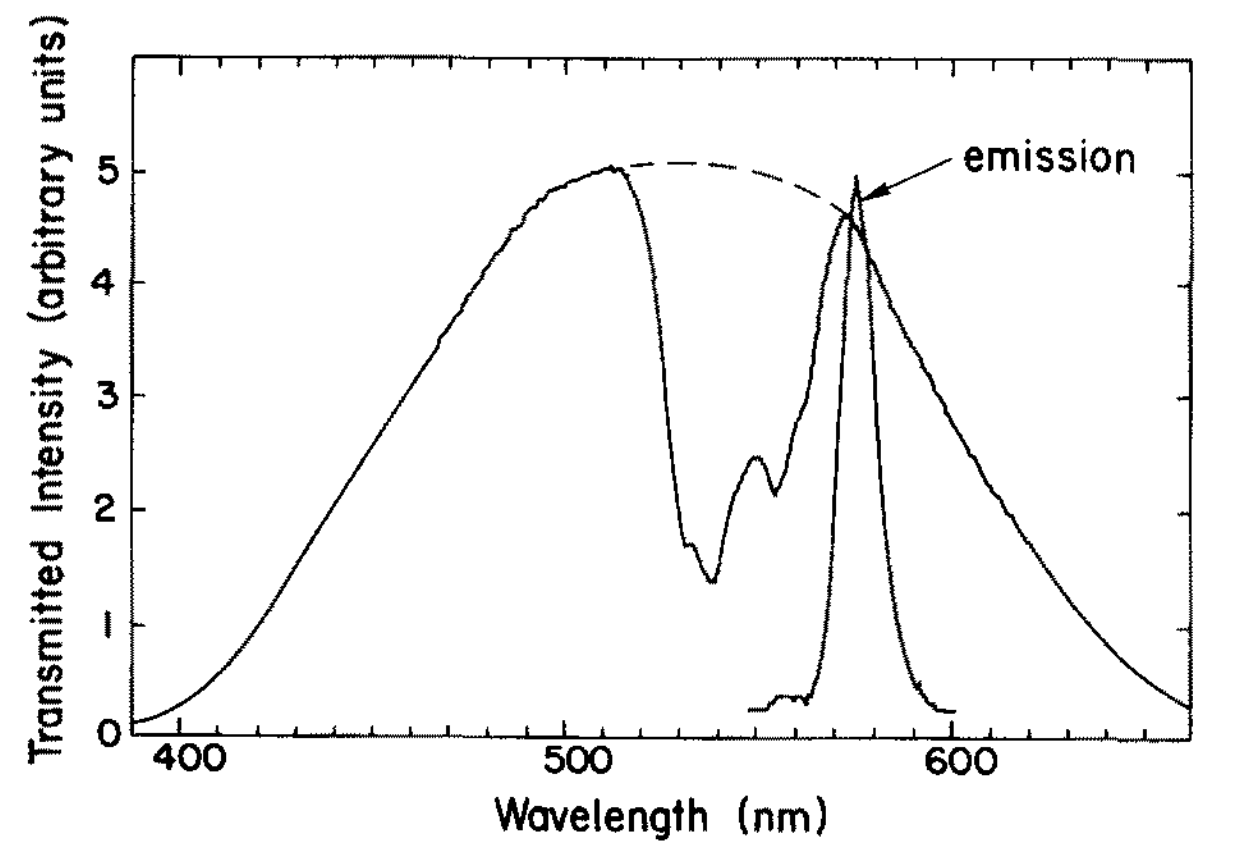
\includegraphics[width=.7\textwidth]{figures/Ba_in_SAr.png}
                \caption{Absorption and emission spectra of neutral Ba in SAr at 10~K.  \cite{SAr}}
\label{fig:BaSAr}
\end{figure}

Energy level transition probabilities can also be affected in a matrix, e.g., spin-forbidden transitions can become more significant via the heavy atom effect.  If electronic potential energy curves cross each other, non-radiative transitions can become allowed for otherwise forbidden transitions. \cite{crepin}  Effects like these could aid in observation of the Ba/Ba\textsuperscript{+}, e.g. by improving decay rates out of metastable D states, or they could reduce detectability, e.g. if a non-radiative decay competes with the fluorescence channel.

%The detectability of a single atom/ion can depend greatly on [these]...

\section{5-level System}
\label{sec:model}

%\section{6-level System}

%Neutral Ba in vacuum is a 5-level system.  However, solving a 6-level system is helpful in modeling matrix-isolated Ba, where another state could be reached after excitation, e.g. decay into a \textsuperscript{3}P state.  The set of rate equations for this system is shown in Eqn. \ref{eqn:rateEqn}:

\emph{\color{gray}is for 6-level, but could prolly just drop 6th in explanation of \textbf{iterative (numerical) solution to...}:}

\begin{equation}
\begin{aligned}
\frac{dN_1}{dt} &= - w_{12}N_{1} + a_{21}N_{2} + a_{31}N_{3} + a_{41}N_{4} + a_{51} N_{5} + a_{61}N_{6} \\
\frac{dN_2}{dt} &= w_{12}N_{1} - N_{2}(a_{21} + a_{23} + a_{24} + a_{25} + a_{26}) \\
\frac{dN_3}{dt} &= a_{23}N_{2} - a_{31}N_{3} \\
\frac{dN_4}{dt} &= a_{24}N_{2} - a_{41}N_{4} \\
\frac{dN_5}{dt} &= a_{25}N_{2} - a_{51}N_{5} \\
\frac{dN_6}{dt} &= a_{26}N_{2} - a_{61}N_{6}
\end{aligned}
\label{eqn:rateEqn}
\end{equation}

\section{Fluorescence Efficiency}
\label{sec:fluorEff}

Fluorescence efficiency, $\epsilon_{f}$, is the ratio of fluorescence photons emitted to excitations into the fluorescing state.  This becomes less than one when there are paths out of the excited state other than the one which emits the photon being measured, e.g. the $\epsilon_{f}$ of Ba in vacuum is about 99.7\%, not quite 1 due to about 1 in 330 decays from the P state into a metastable D state rather than back to ground.  $\epsilon_{f}$ can be calculated by Eqn. \ref{eqn:flueEff}:

\begin{equation}
\epsilon_{f} = \frac{f}{w_{12} \epsilon_{c}} = \frac{f h \nu}{\sigma I \epsilon_{c}}
\label{eqn:flueEff}
\end{equation}

\noindent
where $f$ is the number of fluorescence photons observed per atom per second, $w_{12}$ is the excitation rate, $\epsilon_{c}$ is the collection efficiency of the system, $\sigma$ is the cross section for the excitation interaction, $I$ is the laser intensity, and $h \nu$ is the excitation photon energy.  $\sigma$ can be measured by experiment, and the remaining parameters are easily calculated to produce a measurement of $\epsilon_{f}$ \emph{/color
{gray}those statements are dumb, and do you want to ref brian for measuring the Ba $\sigma$?}.